\section*{Tarea 3: Control de formaciones}
\addcontentsline{toc}{section}{Tarea 3: Control de formaciones}

El objetivo de esta tarea es implementar un sistema de control de formaciones
basado en un esquema \textit{líder--seguidores}, donde un robot maestro
define la trayectoria global y tres robots esclavos mantienen posiciones
relativas fijas respecto de él. Para ello se han desarrollado dos controladores
progresivos: un \textbf{controlador básico de formación}, y un
\textbf{controlador coordinado} más avanzado que incorpora la velocidad del líder
y una dinámica más estable.

Esta tarea constituye la base para la futura integración con esquemas de
evitación de obstáculos, que se abordarán en la siguiente fase de la práctica.

\subsection*{1. Descripción del experimento}
\addcontentsline{toc}{subsection}{1. Descripción del experimento}

El escenario está compuesto por cuatro robots \textit{Khepera IV} simulados
en \textit{CoppeliaSim}. Uno de ellos actúa como \textit{líder} y los otros
tres como \textit{seguidores}. El líder recibe comandos de velocidad a través
del tópico \texttt{/master\_khepera\_iv/cmd\_vel}, mientras que los seguidores
son gobernados por los controladores implementados en esta tarea.

Cada robot publica su pose mediante el tópico
\texttt{/robot\_pose}, que contiene un mensaje de tipo
\texttt{geometry\_msgs/msg/Pose}. El controlador de formación suscribe
la pose del líder y de los tres seguidores, y publica las velocidades
lineal y angular de cada esclavo en los tópicos:

\begin{itemize}
    \item \texttt{/slave\_1\_khepera\_iv/cmd\_vel}
    \item \texttt{/slave\_2\_khepera\_iv/cmd\_vel}
    \item \texttt{/slave\_3\_khepera\_iv/cmd\_vel}
\end{itemize}

En la Figura \ref{fig:t3.formaciones} se ilustran algunas de las
formaciones utilizadas.

%\begin{figure}[H]
%    \begin{center}
%    \includegraphics[scale=0.22]{Images/tarea3/formacion_cross.png}
%    \includegraphics[scale=0.22]{Images/tarea3/formacion_line.png}
%    \caption{\label{fig:t3.formaciones} Ejemplos de formaciones utilizadas en la Tarea 3.}
%    \end{center}
%\end{figure}

\subsection*{2. Controlador de formación básico}
\addcontentsline{toc}{subsection}{2. Controlador de formación básico}

El primer controlador desarrollado, denominado \texttt{formation\_controller},
implementa un esquema sencillo basado en la persecución de puntos objetivo
definidos a partir de la pose del líder. Cada seguidor persigue una posición
relativa fija \((x_{\text{rel}},y_{\text{rel}})\) expresada en coordenadas
polare–angulares mediante un radio \(r\) y un ángulo \(\beta\).

La posición deseada para cada seguidor se calcula como:

\begin{equation}
\begin{aligned}
x_d &= x_L + r\cos(\theta_L + \beta), \\
y_d &= y_L + r\sin(\theta_L + \beta),
\end{aligned}
\label{eq:t3_basic_target}
\end{equation}

donde \((x_L,y_L,\theta_L)\) es la pose del líder.

El error de posición es:



\[
e_x = x_d - x_s, \qquad e_y = y_d - y_s,
\]



y la dirección deseada se obtiene mediante:



\[
\theta_d = \operatorname{atan2}(e_y, e_x).
\]



El controlador aplica dos modos:

\begin{itemize}
    \item \textbf{Control de posición}: si la distancia al objetivo es mayor que un umbral.
    \item \textbf{Control de orientación}: una vez alcanzado el punto, el seguidor iguala su orientación con la del líder.
\end{itemize}

Las velocidades se calculan como:



\[
v = k_f \, \|e\|, \qquad
\omega = k_\theta (\theta_d - \theta_s),
\]



con saturaciones para garantizar estabilidad.

Este controlador permite mantener formaciones simples, pero no incorpora
información sobre la velocidad del líder, lo que puede generar movimientos
bruscos cuando el líder cambia de dirección.

\subsection*{3. Controlador de formación coordinado}
\addcontentsline{toc}{subsection}{3. Controlador de formación coordinado}

Para mejorar la estabilidad y coherencia dinámica del sistema, se ha
implementado un segundo controlador más avanzado:
\texttt{coordinated\_formation\_controller}. Este controlador incorpora:

\begin{itemize}
    \item la velocidad lineal y angular del líder,
    \item un control reactivo en el marco del robot,
    \item modos estacionario y dinámico,
    \item restricciones para evitar retrocesos,
    \item saturaciones suaves.
\end{itemize}

\paragraph{Posición objetivo}

La posición deseada se define mediante una transformación rígida:

\begin{equation}
\begin{pmatrix}
x_d \\ y_d
\end{pmatrix}
=
\begin{pmatrix}
x_L \\ y_L
\end{pmatrix}
+
\begin{pmatrix}
\cos\theta_L & -\sin\theta_L \\
\sin\theta_L & \cos\theta_L
\end{pmatrix}
\begin{pmatrix}
x_{\text{rel}} \\ y_{\text{rel}}
\end{pmatrix}.
\label{eq:t3_target}
\end{equation}

\paragraph{Control cinemático}

El error en el marco del robot es:



\[
\begin{pmatrix}
e_{x,r} \\ e_{y,r}
\end{pmatrix}
=
\begin{pmatrix}
\cos\theta_s & \sin\theta_s \\
-\sin\theta_s & \cos\theta_s
\end{pmatrix}
\begin{pmatrix}
e_x \\ e_y
\end{pmatrix}.
\]



El controlador dinámico es:

\begin{equation}
v = v_L + k_x\, e_{x,r}, \qquad
\omega = w_L + k_y\, e_{y,r},
\label{eq:t3_control}
\end{equation}

con la restricción:



\[
e_{x,r} < 0 \;\Rightarrow\; v = 0.
\]



\paragraph{Modos de operación}

\begin{itemize}
    \item \textbf{Modo estacionario}: si el líder está parado o aún no ha publicado velocidades.
    \item \textbf{Modo dinámico}: si el líder está en movimiento.
\end{itemize}

Ambos modos incluyen saturaciones:



\[
v \leftarrow \operatorname{clamp}(v,\,-v_{\max},\,v_{\max}), \qquad
\omega \leftarrow \operatorname{clamp}(\omega,\,-\omega_{\max},\,\omega_{\max}).
\]



\subsection*{4. Implementación en ROS2}
\addcontentsline{toc}{subsection}{4. Implementación en ROS2}

Se han desarrollado dos nodos:

\begin{itemize}
    \item \texttt{formation\_controller}: controlador básico.
    \item \texttt{coordinated\_formation\_controller}: controlador avanzado.
\end{itemize}

Los parámetros del controlador avanzado se cargan desde:

\begin{verbatim}
coordinated_formation_controller:
  ros__parameters:
    formation_type: "cross"
    kx: 0.5
    ky: 1.2
    dist_stationary_thresh: 0.03
    dist_dynamic_thresh: 0.12
    v_max: 0.15
    w_max: 1.0
    leader_v_eps: 0.01
    leader_w_eps: 0.01
\end{verbatim}

\subsection*{5. Resultados}
\addcontentsline{toc}{subsection}{5. Resultados}

En la Figura \ref{fig:t3.traj} se muestra la trayectoria obtenida durante
la ejecución del controlador avanzado. Los seguidores convergen a sus
posiciones relativas y mantienen la formación mientras el líder se desplaza.

SIMPLE
\begin{figure}[H]
    \begin{center}
    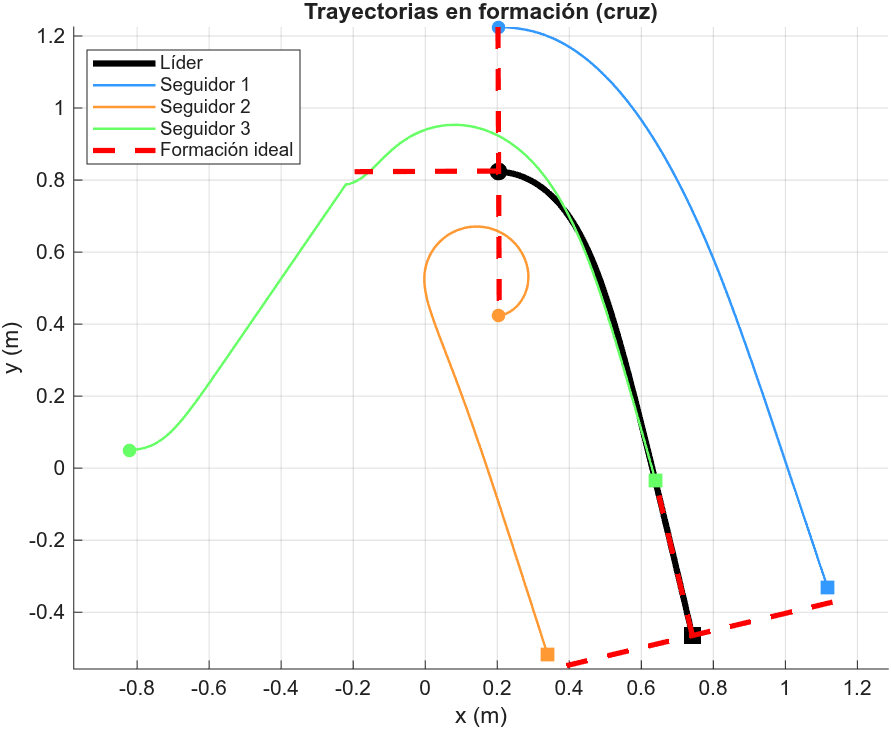
\includegraphics[scale=0.85]{Images/tarea3/coordinated_formation_crossSimple.png}
    \caption{\label{fig:t3.cross_coordinado} Coordinado simple en cruz.}
    \end{center}
\end{figure}

\begin{figure}[H]
    \begin{center}
    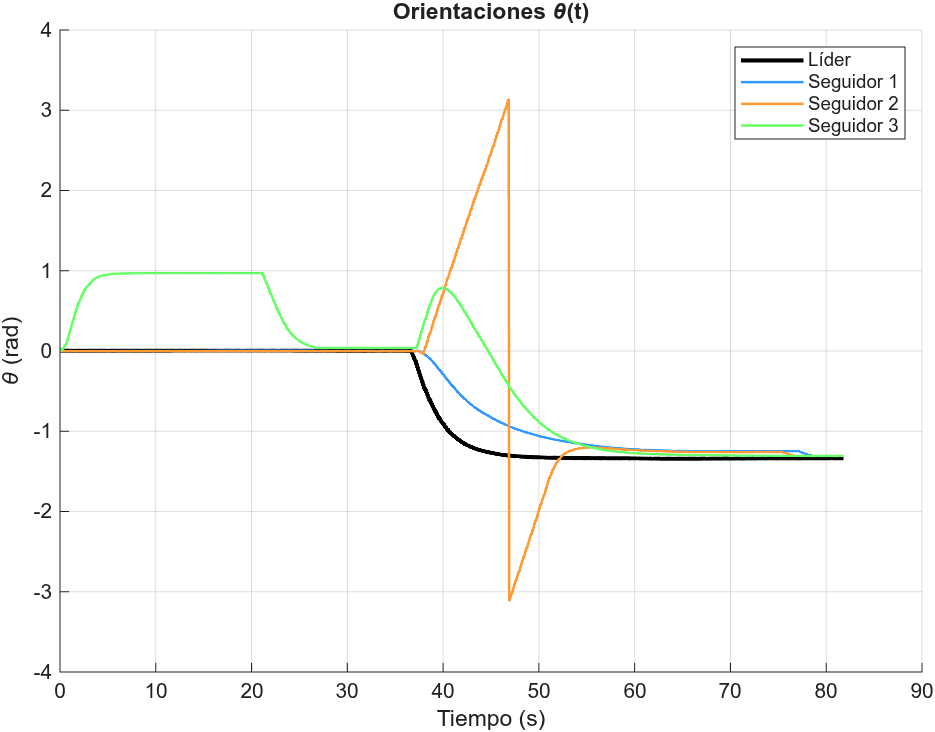
\includegraphics[scale=0.85]{Images/tarea3/coordinated_orient_formation_crossSimple.png}
    \caption{\label{fig:t3.cross_coordinado_orient} Coordinado simple en cruz orientaciones.}
    \end{center}
\end{figure}

\begin{figure}[H]
    \begin{center}
    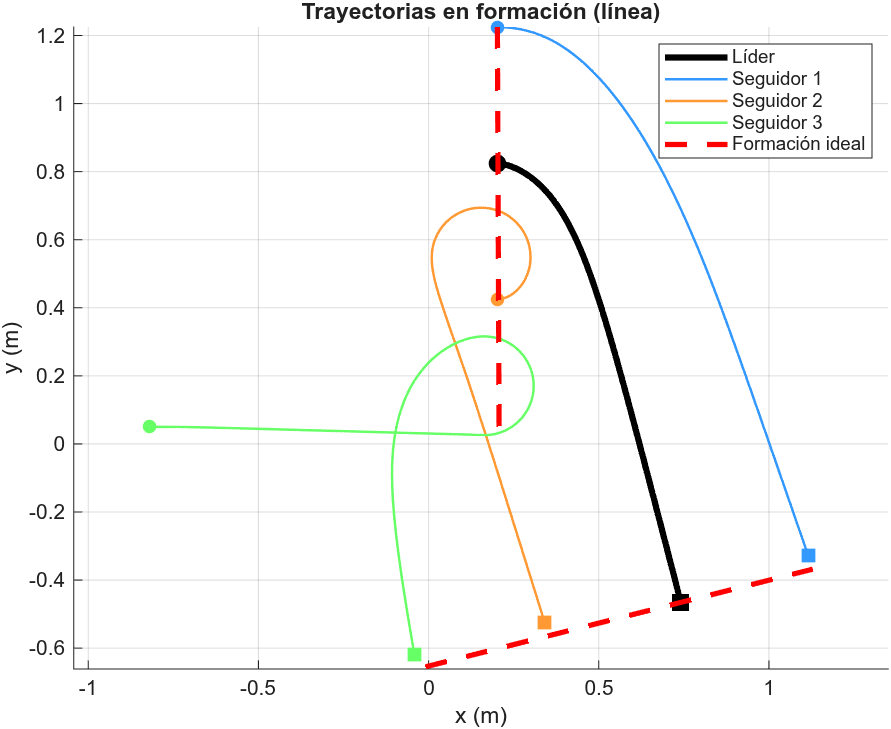
\includegraphics[scale=0.85]{Images/tarea3/coordinated_formation_lineSimple.png}
    \caption{\label{fig:t3.line_coordinado} Coordinado simple en línea.}
    \end{center}
\end{figure}

\begin{figure}[H]
    \begin{center}
    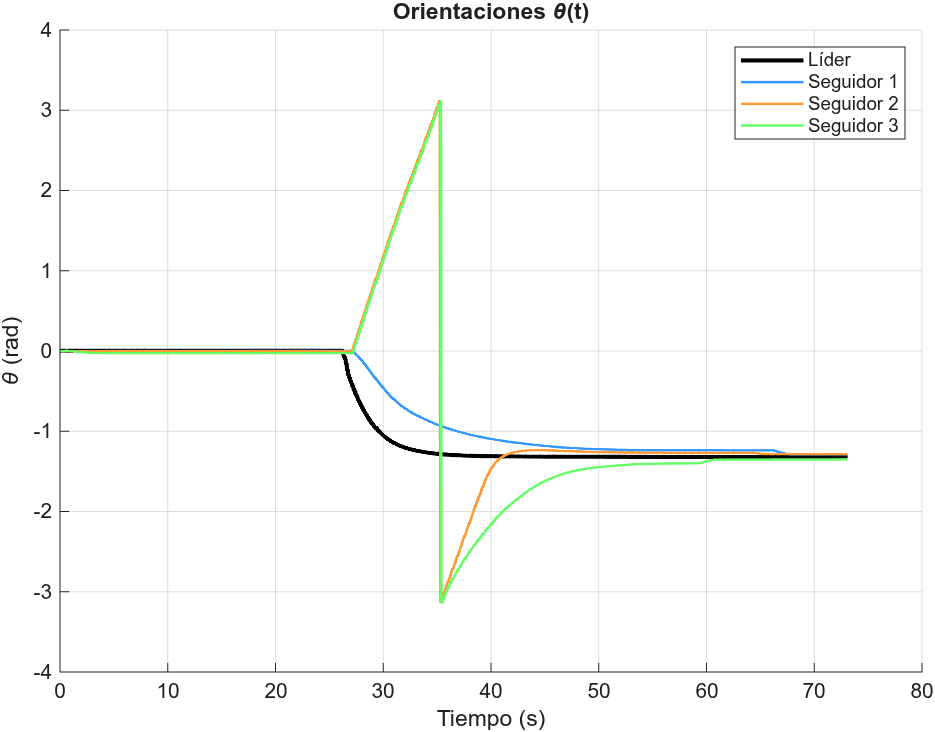
\includegraphics[scale=0.85]{Images/tarea3/coordinated_orient_formation_lineSimple.png}
    \caption{\label{fig:t3.line_coordinado_orient} Coordinado simple en línea orientaciones.}
    \end{center}
\end{figure}

\begin{figure}[H]
    \begin{center}
    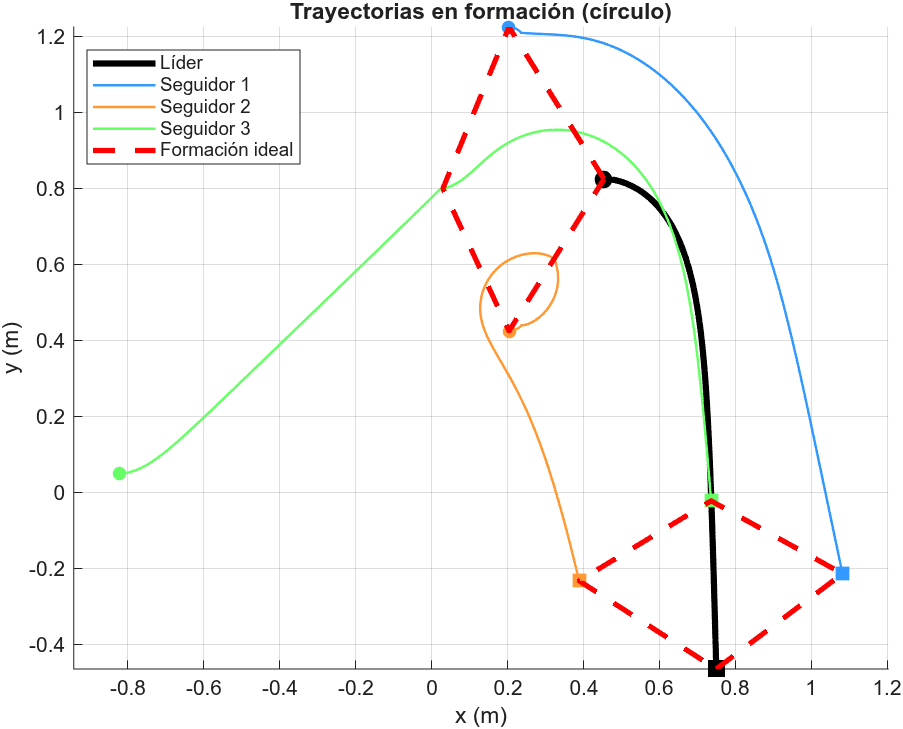
\includegraphics[scale=0.85]{Images/tarea3/coordinated_formation_circleSimple.png}
    \caption{\label{fig:t3.circle_coordinado} Coordinado simple en círculo.}
    \end{center}
\end{figure}

\begin{figure}[H]
    \begin{center}
    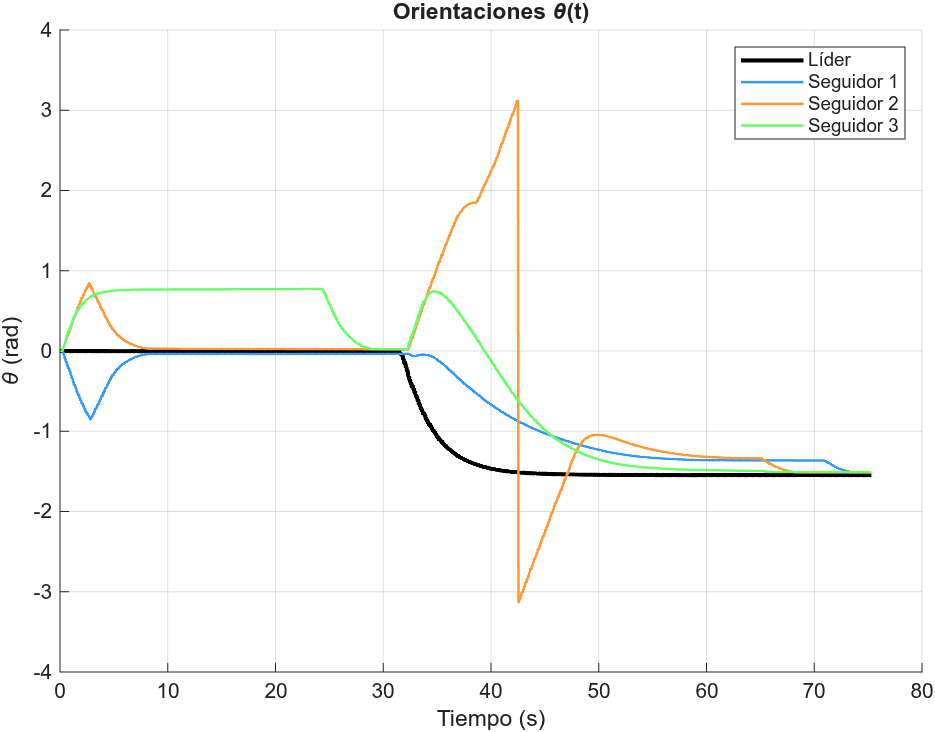
\includegraphics[scale=0.85]{Images/tarea3/coordinated_orient_formation_circleSimple.png}
    \caption{\label{fig:t3.circle_coordinado_orient} Coordinado simple en círculo orientaciones.}
    \end{center}
\end{figure}


COMPLEJO
\begin{figure}[H]
    \begin{center}
    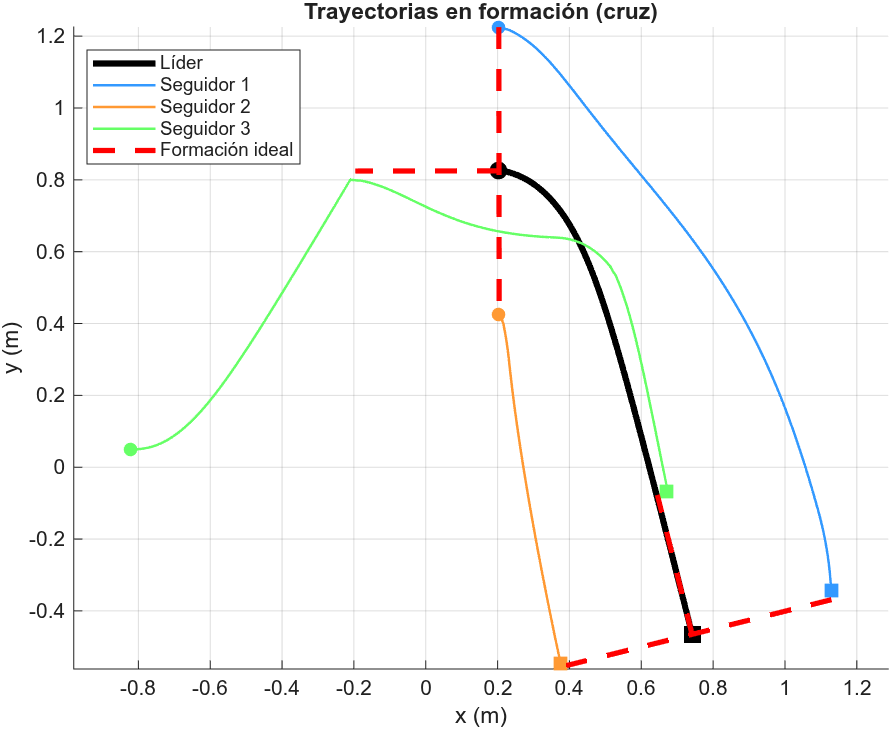
\includegraphics[scale=0.85]{Images/tarea3/coordinated_formation_cross.png}
    \caption{\label{fig:t3.cross_coordinado} Coordinado en cruz.}
    \end{center}
\end{figure}

\begin{figure}[H]
    \begin{center}
    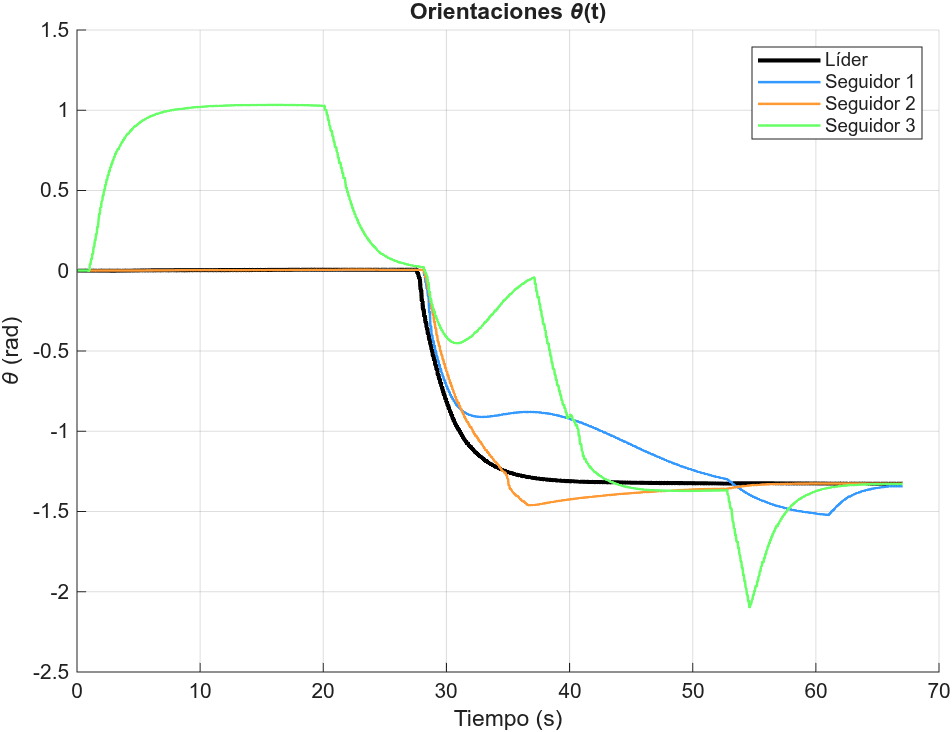
\includegraphics[scale=0.85]{Images/tarea3/coordinated_orient_formation_cross.png}
    \caption{\label{fig:t3.cross_coordinado_orient} Coordinado en cruz orientaciones.}
    \end{center}
\end{figure}

\begin{figure}[H]
    \begin{center}
    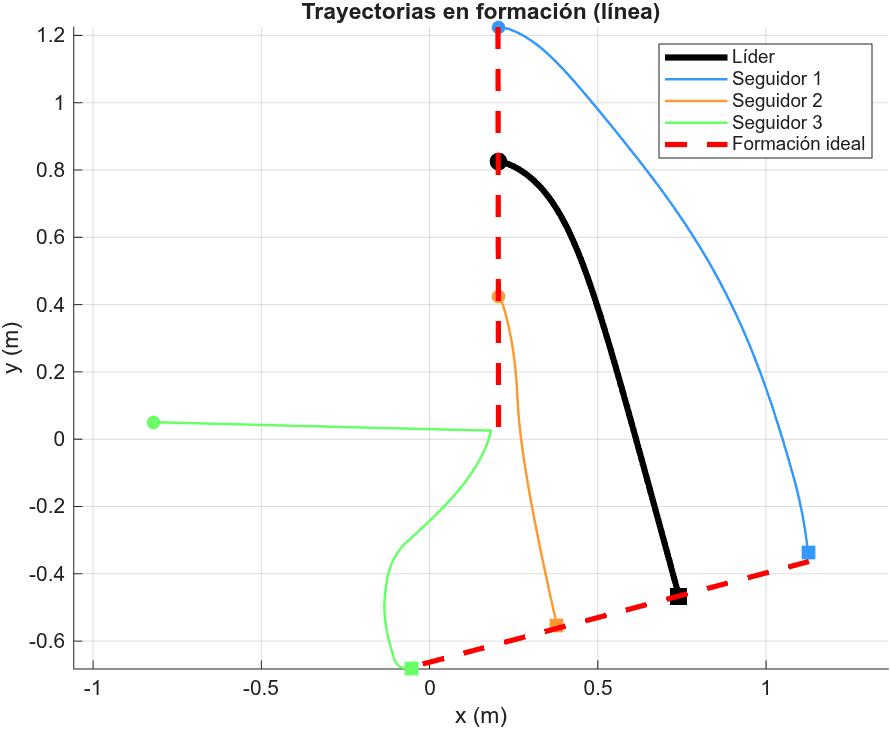
\includegraphics[scale=0.85]{Images/tarea3/coordinated_formation_line.png}
    \caption{\label{fig:t3.line_coordinado} Coordinado en línea.}
    \end{center}
\end{figure}

\begin{figure}[H]
    \begin{center}
    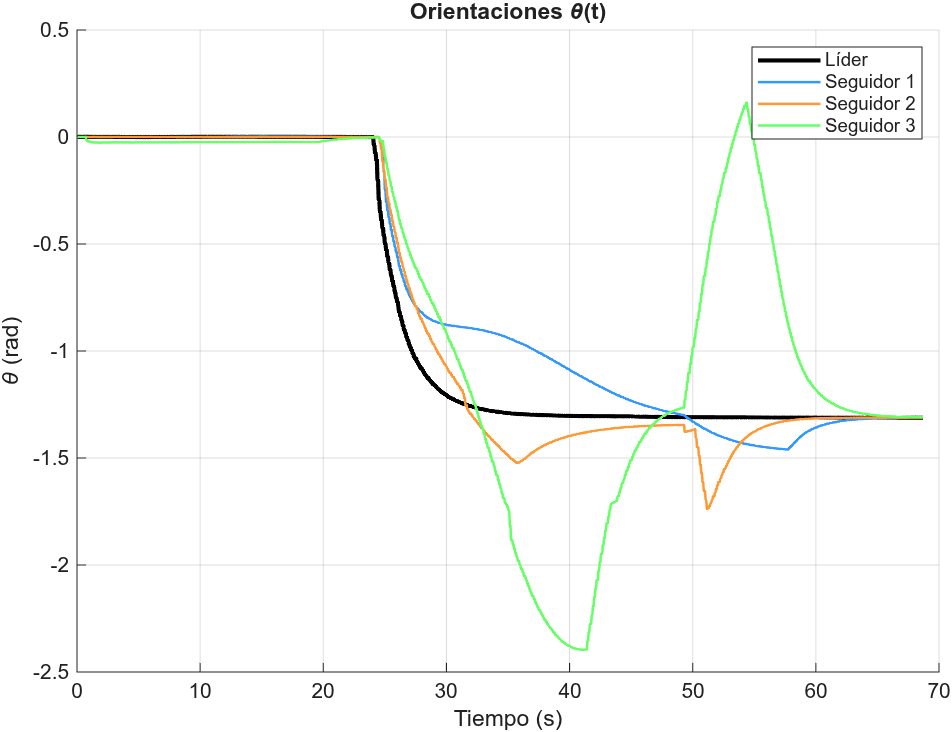
\includegraphics[scale=0.85]{Images/tarea3/coordinated_orient_formation_line.png}
    \caption{\label{fig:t3.line_coordinado_orient} Coordinado en línea orientaciones.}
    \end{center}
\end{figure}

\begin{figure}[H]
    \begin{center}
    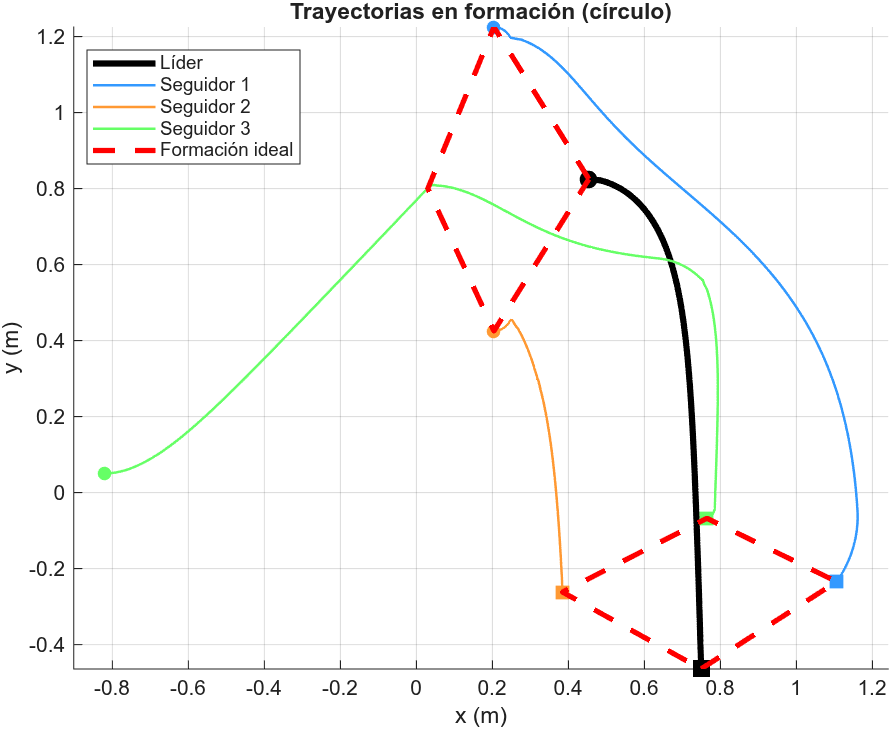
\includegraphics[scale=0.85]{Images/tarea3/coordinated_formation_circle.png}
    \caption{\label{fig:t3.circle_coordinado} Coordinado en círculo.}
    \end{center}
\end{figure}

\begin{figure}[H]
    \begin{center}
    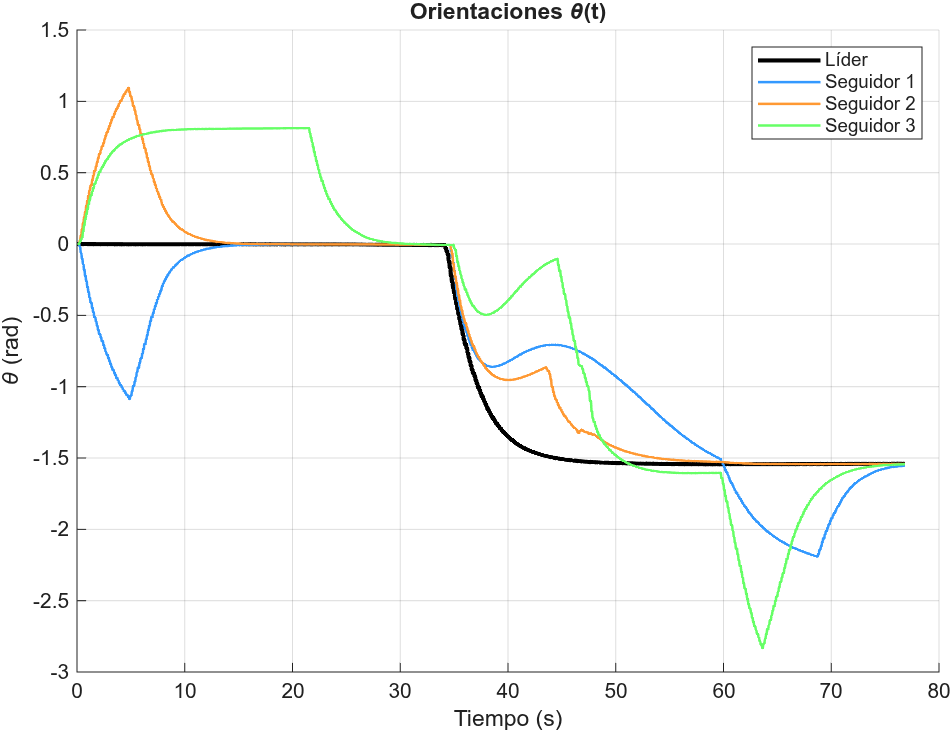
\includegraphics[scale=0.85]{Images/tarea3/coordinated_orient_formation_circle.png}
    \caption{\label{fig:t3.circle_coordinado_orient} Coordinado en círculo orientaciones.}
    \end{center}
\end{figure}

%\begin{figure}[H]
%    \begin{center}
%    
\includegraphics[scale=0.85]{Images/tarea3/traj.png}
%    \caption{\label{fig:t3.traj} Trayectoria del líder y seguidores en formación.}
%    \end{center}
%\end{figure}

En la Figura \ref{fig:t3.vels} se representan las velocidades lineal y angular
de uno de los seguidores.

%\begin{figure}[H]
%    \begin{center}
%    
\includegraphics[scale=0.8]{Images/tarea3/v.png} \\
%    
\includegraphics[scale=0.8]{Images/tarea3/w.png}
%    \caption{\label{fig:t3.vels} Velocidades lineal y angular del seguidor.}
%    \end{center}
%\end{figure}

\subsection*{6. Conclusiones}
\addcontentsline{toc}{subsection}{6. Conclusiones}

Se han implementado dos controladores de formación basados en un esquema
\textit{líder--seguidores}. El controlador básico permite mantener formaciones
geométricas simples, mientras que el controlador coordinado incorpora la
dinámica del líder y proporciona un comportamiento más estable y coherente.

Este trabajo constituye la base para la siguiente fase de la práctica,
donde se integrará un módulo de evitación de obstáculos que permitirá
mantener la formación incluso en entornos no estructurados.
